\chapter{Lecture: 09/05/2025}

\section{Spatiotemporal noisy model}

$$
\dfrac {\partial \phi}{\partial t} = f(\phi) + g(\phi) \xi_m(r,t) + D \mathcal L[\phi] + h(\phi) F(t) + \xi_a(r,t)
$$

\begin{itemize}
\item $f(\phi)$: deterministic part
\item $g(\phi)$: multiplicative noise
\item $D \mathcal L[\phi]$: linear part
\item $h(\phi)$: additive noise
\end{itemize}

L[\phi] is a Laplacian or a integral operator

Examples:

\begin{itemize}
\item
$$
\mathcal L[\phi] = \nabla^2 \phi
$$
\item
$$
\mathcal L[\phi] = -a_0 \nabla^2 \phi - \nabla^4 \phi
$$
\item
$$
\mathcal L[\phi] = -(\nabla^2 + k_0^2)^2 \phi = - (K_0^2 + 2 k_0 \nabla^2 + \nabla^4) \phi
$$
\end{itemize}

\begin{observationblock}
    If we apply the fourier transform of:
    $$
    \mathcal L[\phi] = -(\nabla^2 + k_0^2)^2 \phi = - (K_0^2 + 2 k_0 \nabla^2 + \nabla^4) \phi
    $$

    we get:

    $$
    ... F(\phi)
    $$

\end{observationblock}

$$
\mathcal L[\phi(r)] = \int \phi(r') \omega(r-r') \dd r'
$$

How do we simulate this equation? We can simply obtain the domain and discretize it.

Lattice.based Approximation:

$$
...
$$

Field coupling approximation:

$$
l(\phi_i, \phi_j) = w_i \phi_i + \sum_{j \in nn(i)} w_j \phi_j
$$

For example:

$$
\mathcal L[\phi] = \nabla^2 \phi \approx l(\phi_i, \phi_j) = \dfrac 1{\Delta^2} \sum_{j \in nn(i)} (\phi_j - \phi_i)
$$

If we have a stochastic process which is discrete in time and space, we have:

$$
\left\langle \xi(r,t) \xi(r',t') \right\rangle = sC \left(
    \dfrac{|r-r'|}{d}, \dfrac{|t-t'|}{\tau_c}
\right)
$$

As in the purely temporal noise, $\tau_c$ is a measure of the temporal memory of the noise, $d$ is the spatial memory of the noise.

The spatiotemporal brother of the ornstein-uhlenbeck noise is "Ojalvo e al" noise.

$$
\dfrac{\partial \phi}{\partial t} = a \phi + D \nabla^2 \phi + \xi_{gn}
$$

\begin{observationblock}[Ojalvo e al and the Ornstein-Uhlenbeck process]
    If we set $D = 0$ we have a series of Ornstein-Uhlenbeck processes at each point of the domain.
    $$
    \dfrac{\partial \phi}{\partial t} = a \phi + \xi_{gn}
    $$
\end{observationblock}

Noise induced pattenrs §

$$
\dfrac{\partial \phi}{\partial t} = f(\phi) + g(\phi) \xi_m(r,t) + D \mathcal L[\phi] + ...
$$
\dots

Perturbed Swift-Hohenberg model:

$$
\dfrac{\partial \phi}{\partial t} = a \phi + D \mathcal L[\phi] + \xi_{gn} ...
$$

$$
\dfrac{\partial \phi}{\partial t} = f(\phi) + D \mathcal L[\phi] = a\phi - D (\nabla^2 + k_0^2)^2 \phi
$$

Transitory pattern that disappear.

% \begin{figure}[h]
%     \centering
%     \includegraphics[width=0.5\textwidth]{assets/perturbed_swift_hohenberg_model.png}
%     \caption{Perturbed Swift-Hohenberg model}
%     \label{fig:perturbed_swift_hohenberg_model}
% \end{figure}

Additive noise generate pattenrs

$$
\dfrac{\partial \phi}{\partial t} = a \phi + D \mathcal L[\phi] + \xi_{gn}, \qquad \mathcal L[\phi] = - (\nabla^2 + k_0^2)^2 \phi
$$

Permanent patterning: details change in time.

we can distinguish two cases:

\begin{itemize}
\item $a < 0$ 

\item $a > 0$ 

\end{itemize}

with multiplicative noise it can induce bimodality in the pdf of $\phi$:

% \begin{figure}[h]
%     \centering
%     \includegraphics[width=0.5\textwidth]{assets/pdf_bimodality.png}
%     \caption{Perturbed Swift-Hohenberg model}
%     \label{fig:perturbed_swift_hohenberg_model}
% \end{figure}

$$
\dfrac{\partial \phi}{\partial t} = a \phi - phi^3 + \phi \xi_{gn} + D \mathcal L[\phi]
$$ 

---

A bad model of glaciations

$$
\dd x = [x(a-x^2) + A \cos \Omega t] \dd t
$$

where

\begin{itemize}
\item $x$: is the (normalized) Earth's temperature
\item $A \cos(\Omega t)$: small periodic variations of the solar irradiation. 
\end{itemize}

We have that if $A$ is small, $x(t)$ fluctuates around $+\sqrt(a)$.

The model fails.

Including stochastic noise:

$$
\dd x = [x(a-x^2) + A \cos \Omega t] \dd t + \varepsilon \dd W
$$

where $\varepsilon$ is the noise intensity.

This time we have a white noise, according to:

\begin{itemize}
    \item $\varepsilon$ is small: the noise is negligible
    \item $\varepsilon$ is large: the noise is dominant
\end{itemize}

they finally managed to model the glaciations.

---

\subsubsection{Spatial Stochastic Resonance}

$$
\dfrac{\partial \phi}{\partial t} = a\phi - \phi^3 + D \dfrac{\partial^2 \phi}{\partial x^2} + F(t) + \varepsilon \xi_{gn}
$$

\todo{check the formula}

\dots

\newpage

\chapter{Discrete Time Markov Chains}

We consider the case where the time is a subset of the integers ($t \subset \mathbb{Z}$ or $t \subset \mathbb{N}_0$)

The state space is a finite set $S = \{s_1, s_2, \dots, s_N\}$
\vspace{0.4em}
$$
P \{ x(t+1) | x(0), x(1), \cdots, x(t) \} = P \{ x(t+1) | x(t) \}
$$

The probability that the process in $t+1$ is $\sigma$ is the sum of the probability that the process in $t$ is $\delta$ and the probability that the process in $t+1$ is $\sigma$ given that the process in $t$ is $\delta$.
\vspace{0.4em}
$$
P \{ x(t+1) = \sigma \} = \sum_{\delta \in S} P \{ x(t + 1) = \sigma | x(t) = \delta \} P \{ x(t) = \delta \}
= \sum_{\delta \in S} P \{ x(t) = \delta \} \theta_{\delta \sigma}
$$

with $\theta_{\delta \sigma} \in [0, 1]$.

So we have:
\vspace{0.4em}
$$
P_{\sigma}(t+1) = \sum_{\delta \in S} P_{\delta}(t) \theta_{\delta \sigma}
\quad \Rightarrow \quad
P(t+1) = P(t) \Theta(t)
$$

Where $P(t) = [P_1(t), P_2(t), \cdots, P_N(t)]$ is the probability vector at time $t$ and $\Theta(t)$ is the transition matrix at time $t$.

We have:
$$
P(1) = P(0) \Theta
,\quad
P(2) = P(1) \Theta = P(0) \Theta^2
,\quad
P(3) = P(2) \Theta = P(0) \Theta^3
, \quad \cdots
$$

We can write:
$$
P(t) = P(0) \Theta^t = P(0) \prod_{q = 0}^{t-1} \Theta(q)
$$

We have two properties:

$$
\sum_{\sigma \in S} \theta_{\delta \sigma} = 1
, \qquad \quad
\sum_{\delta \in S} P_{\delta}(t) = 1
$$

So we have:

$$
P_{\sigma}(t + 1) = \sum_{\delta \in S} P_{\delta}(t) \theta_{\delta \sigma}
\quad \Rightarrow \quad
\sum_{\sigma \in S} P_{\sigma}(t + 1) = \sum_{\sigma} \sum_{\delta} P_{\delta}(t) \theta_{\delta \sigma}
= \sum_{\delta} P_{\delta}(t) \sum_{\sigma} \theta_{\delta \sigma}
= 1
$$

So

\missing{something}

---

Let's consider again the discrete time Markov chain.

$$
P_{\sigma}(t+1) = P(t) \Theta \quad \Rightarrow \quad P(t) = P(0) \Theta^t
$$

\dots

$$
P^\infty = P^\infty \Theta
$$

Let's study the eigenvalues of $\Theta$:

$$
\Theta v = \lambda v
$$

$$
\sum_{\sigma} \theta_{\delta \sigma} = 1
$$

(... non ho capito perchè ma l'autovettore di $\Theta$ è formato da tutti 1 ...)

If the multiplicity of the eigenvalue is more than 1, we have multiple solutions to our system.


\begin{tipsblock}

    Sometimes this equation is written as:
    $$
    P_a(t+1) = \sum_{s \in S} W_{as} P_s(t)
    $$
    where $W_{as}$ ...
\end{tipsblock}

\missing{something}

---

\begin{exampleblock}[Simple markov chain]

    The simplest markov chain is the one with only one state, with a transition with probability $1$ from the state to itself.

    $$
    P(0) = [1], \qquad P(t) = [1]
    $$

    ---

    Another simple markov chain is the one with two states, with a transition with probability $1$ from the state $s_0$ to the state $s_1$ and with probability $1$ from the state $s_1$ to the state $s_1$ itself.

    \begin{figure}[H]
        \centering
        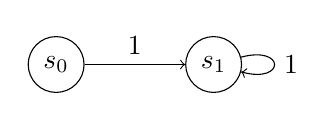
\begin{tikzpicture}
            \node[circle,draw] (s1) at (0, 0) {$s_0$};
            \node[circle,draw] (s2) at (2, 0) {$s_1$};
            \draw[->] (s1) to node[above] {$1$} (s2);
            \draw[->] (s2) to[loop right] node[right] {$1$} (s2);
        \end{tikzpicture}
    \end{figure}

    We have the situation below:
    
    $$
    P(0) = [1, 0], \qquad P(t) = [0, 1]
    $$

    A more complex example is the following:

    \begin{figure}[H]
        \centering
        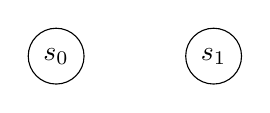
\begin{tikzpicture}
            \node[circle,draw] (s1) at (0, 0) {$s_0$};
            \node[circle,draw] (s2) at (2, 0) {$s_1$};
        \end{tikzpicture}
    \end{figure}

    \todo{add the transitions in the figure}

    $$
    P_0(t+1) = \theta_{00} P_0(t) +  P_1(t) \theta_{10}
    $$

    $$
    P_1(t) = 1- P_0(t) \quad \Rightarrow \quad P_0(t+1) = \theta_{00} P_0(t) + \theta_{10} (1-P_0(t))
    $$
    
    $$
    \boxed{P_0(t+1) = (\theta_{00} - \theta_{10}) P_0(t) + \theta_{10}}
    $$
\end{exampleblock}

If we have a case like:

$$
x(t+1) = ax + b
$$

then we have a term $b$ that don't allow us to use the resolution formula we are used to ($x(t) = x(0) a^t $), but ...

\dots

\begin{figure}[H]
    \centering
    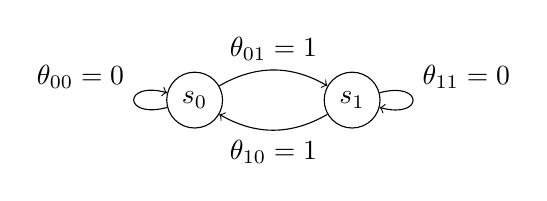
\begin{tikzpicture}
        \node[circle,draw] (s1) at (0, 0) {$s_0$};
        \node[circle,draw] (s2) at (2, 0) {$s_1$};
        % loop on s0
        \draw[->] (s1) to[loop left] node[left, yshift=0.3cm] {$\theta_{00} = 0$} (s1);
        % transition from s0 to s1
        \draw[->] (s1) to[bend left=30] node[above] {$\theta_{01} = 1$} (s2);
        % loop on s1
        \draw[->] (s2) to[loop right] node[right, yshift=0.3cm] {$\theta_{11} = 0$} (s2);
        % transition from s1 to s0
        \draw[->] (s2) to[bend left=30] node[below] {$\theta_{10} = 1$} (s1);
    \end{tikzpicture}
\end{figure}

$$
\begin{array}{c}
P(0) = [1, 0] = x(0) = 0
\\[0.2em]
P(1) = [0, 1] = x(1) = 1
\\[0.2em]
P(2) = [1, 0] = x(2) = 0
\\[0.2em]
\vdots
\end{array}
$$

Which is periodic.

\dots

\begin{exampleblock}[Bora example]

Let's consider the case of Bora in Trieste. We have two states: $B$ and $N$.

\begin{figure}[H]
    \centering
    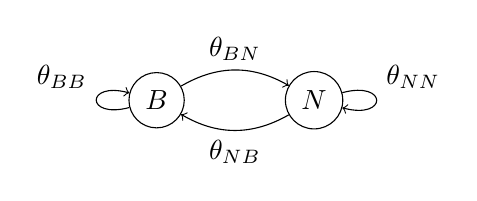
\begin{tikzpicture}
        \node[circle,draw] (s1) at (0, 0) {$B$};
        \node[circle,draw] (s2) at (2, 0) {$N$};
        % loop on s0
        \draw[->] (s1) to[loop left] node[left, yshift=0.3cm] {$\theta_{BB}$} (s1);
        % transition from s0 to s1
        \draw[->] (s1) to[bend left=30] node[above] {$\theta_{BN}$} (s2);
        % loop on s1
        \draw[->] (s2) to[loop right] node[right, yshift=0.3cm] {$\theta_{NN}$} (s2);
        % transition from s1 to s0
        \draw[->] (s2) to[bend left=30] node[below] {$\theta_{NB}$} (s1);
    \end{tikzpicture}
\end{figure}
\vspace{-1em}
We have the following transition probabilities:

$$
\begin{array}{ccc}
\theta_{BB} \approxeq \dfrac{NT^{BB}}{N_B}
& \qquad &
\theta_{BN} \approxeq \dfrac{NT^{BN}}{N_B}
\\[1em]
\theta_{NB} \approxeq \dfrac{NT^{NB}}{N_N}
& \qquad &
\theta_{NN} \approxeq \dfrac{NT^{NN}}{N_N}
\end{array}
$$

This model is actually too artificious, because the transition probabilities are not independent, and also depends on other parameters, like the temperature.
\end{exampleblock}

The most natural representatiin of Markov Chains are oriened graphs.

Let's consider a 4 states model:

\begin{figure}[H]
    \centering
    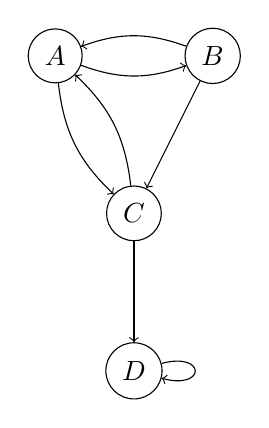
\begin{tikzpicture}
        \node[circle,draw] (A) at (0, 0) {$A$};
        \node[circle,draw] (B) at (2, 0) {$B$};
        \node[circle,draw] (C) at (1, -2) {$C$};
        \node[circle,draw] (D) at (1, -4) {$D$};
        \draw[->] (A) to[bend right=20] (B);
        \draw[->] (A) to[bend right=20] (C);
        \draw[->] (B) to[bend right=20] (A);
        \draw[->] (B) to (C);
        \draw[->] (C) to (D);
        \draw[->] (C) to[bend right=20] (A);
        \draw[->] (D) to[loop right] (D);
    \end{tikzpicture}
\end{figure}

...boh...